
\documentclass{article}
\usepackage{enumitem}
\usepackage{graphicx}

\begin{document}


\title{Xflow Research: Analyzing Departmental Excellence, Professional Practices and Working Procedures}
\author{}
\date{}
\maketitle


\section*{Introduction}

\subsection*{Company Overview}
Xflow Research is a leading software company in Pakistan, providing research and development services in the networking domain. The company was founded in 2012 and has since grown to become a trusted partner for telecommunications companies, cloud providers, and enterprise customers around the world.
\subsection*{Xflow Research's Expertise and Services}
Xflow Research's expertise in NFV, SDN, OpenStack, and cloud computing enables the company to help customers develop and deploy innovative networking solutions. The company's services are followed in the upcoming content.

\subsection*{Consulting and Design Services}

\begin{itemize}
  \item NFV consulting and design: Xflow helps customers to plan and design their NFV infrastructure, taking into account their specific needs and requirements.
  \item SDN consulting and design: Xflow helps customers to design and deploy SDN networks, enabling them to improve network agility and efficiency.
  \item OpenStack consulting and design: Xflow helps customers to deploy and manage OpenStack clouds, providing them with a scalable and flexible cloud infrastructure.
  \item Cloud computing consulting and design: Xflow helps customers to migrate their workloads to the cloud and to develop cloud-native applications.
\end{itemize}

\hfill \break

\subsection*{Development Services}

In addition to its consulting and design services, Xflow Research also offers a range of development services, including:

\begin{itemize}
  \item Custom software development: Xflow develops custom software solutions to meet the specific needs of its customers.
  \item Open source software development: Xflow contributes to and maintains a number of open source software projects, including OpenStack and ONAP.
  \item Product development: Xflow develops and sells its own networking products, such as its SDN controller and NFV management platform.
\end{itemize}

\subsection*{Commitment to Professional Practices}
Xflow Research is committed to following professional practices in all departments to ensure efficient and effective operations. These practices are designed to help the company meet its business goals, deliver high-quality products and services to customers, and protect its IT assets.

\subsection*{Analyzing Professional Practices}
This document provides an analysis of the key professional practices followed by each department at Xflow Research. It also includes recommendations for how the company can further improve its professional practices.

\subsection*{Recommendations for Improvement}
The following sections of this document will discuss the professional practices followed by the marketing, development, project management, and IT departments at Xflow Research.

\subsection*{Departmental Professional Practices}
Xflow Research has four main departments: marketing, development, project management, and IT. Each department follows a set of professional practices to ensure that the company operates efficiently and effectively.

\hfill \break
\hfill \break
\hfill \break

\section{Development Department}

\subsection{Key Professional Practices}

\begin{itemize}
  \item \textbf{Agile development methodology:} The development team uses an agile development methodology to deliver products and services quickly and efficiently. This methodology involves breaking down large projects into smaller, more manageable tasks that can be completed in short sprints.
  \item \textbf{Continuous integration and continuous delivery (CI/CD):} The development team uses CI/CD practices to automate the build, test, and deployment process. This helps to ensure that products and services are delivered to customers quickly and with high quality.
  \item \textbf{Code quality:} The development team is committed to writing clean, well-organized, and maintainable code. This helps to reduce the number of bugs and makes it easier to add new features and functionality in the future.
\end{itemize}

\subsection{Recommendations}

\begin{itemize}
  \item \textbf{Adopt new technologies, such as cloud computing and DevOps, to improve the development and deployment process.} Cloud computing can provide the team with access to scalable and reliable computing resources on demand. DevOps practices can help the team to automate tasks and streamline the development and deployment process.
  \item \textbf{Implement a quality assurance (QA) process to ensure that products and services meet the required quality standards.} The QA process should include unit testing, integration testing, and system testing.
  \item \textbf{Encourage developers to contribute to open source projects to gain new skills and stay up-to-date on the latest technologies.} Contributing to open-source projects can help developers to learn new technologies and best practices. It can also help the team to build relationships with other developers in the community.
\end{itemize}

\section{Marketing Department}

\subsection{Key Professional Practices}

\begin{itemize}
  \item \textbf{Data-driven decision making:} The marketing team uses data and analytics to inform their decision-making process. This ensures that their campaigns are targeted to the right audience and are effective in driving results.
  \item \textbf{Customer-centric approach:} The marketing team is focused on understanding and meeting the needs of their customers. They conduct regular market research and customer surveys to gather feedback and identify new opportunities.
  \item \textbf{Creativity and innovation:} The marketing team is always looking for new and innovative ways to promote Xflow's products and services. They use a variety of channels, including social media, content marketing, and email marketing, to reach their target audience.
\end{itemize}

\subsection{Recommendations}

\begin{itemize}
  \item \textbf{Invest in marketing automation tools to streamline marketing processes and improve efficiency.} This could include tools for email marketing, social media management, and marketing analytics.
  \item \textbf{Develop a content marketing strategy to create and distribute valuable content that attracts and engages potential customers.} This could include blog posts, articles, infographics, and videos.
  \item \textbf{Experiment with new marketing channels, such as social media advertising and influencer marketing.} These channels can help to reach a wider audience and generate leads.
\end{itemize}

\section{Project Management Department}

\subsection{Key Professional Practices}

\begin{itemize}
  \item \textbf{Project planning:} The project management team works with stakeholders to develop detailed project plans. These plans include timelines, budgets, and resource allocation.
  \item \textbf{Risk management:} The project management team identifies and assesses risks to the project and develops mitigation strategies.
  \item \textbf{Communication:} The project management team communicates regularly with stakeholders to keep them updated on the progress of the project and to address any concerns.
\end{itemize}

\subsection{Recommendations}

\begin{itemize}
  \item \textbf{Implement a project management tool to track progress, manage resources, and communicate with stakeholders.} This could include tools such as Jira, Asana, or Trello.
  \item \textbf{Train project managers on best practices in project management, such as risk management and change management.} This could be done through in-house training or by sending project managers to external training courses.
  \item \textbf{Establish a project management center of excellence to share knowledge and best practices across the company.} This could involve creating a repository of project management templates and tools or holding regular workshops and training sessions.
\end{itemize}

\section{IT Department}

\subsection{Key Professional Practices}

\begin{itemize}
  \item \textbf{Service level agreements (SLAs):} The IT department has SLAs in place with other departments at the company to ensure that IT services are delivered to a certain level of quality. SLAs typically specify things like uptime, response time, and resolution time.
  \item \textbf{Change management:} The IT department has a change management process in place to ensure that changes to IT systems are made in a controlled and coordinated manner. This helps to reduce the risk of disruptions and outages.
  \item \textbf{Security:} The IT department implements security measures to protect the company's IT systems from cyber-attacks. This includes measures such as firewalls, intrusion detection systems, and data encryption.
\end{itemize}

\subsection{Recommendations}

\begin{itemize}
  \item \textbf{Implement a cloud migration strategy to move the company's IT infrastructure to the cloud.} The cloud can provide a number of benefits, including scalability, reliability, and cost savings.
  \item \textbf{Adopt a zero-trust security model.} A zero-trust security model assumes that no user or device can be trusted by default. This requires all users and devices to authenticate and authorize themselves before they are allowed to access the company's IT systems.
  \item \textbf{Invest in training and development for IT staff.} This will help to ensure that IT staff have the skills and knowledge they need to keep the company's IT systems secure and up-to-date.
\end{itemize}

\textbf{By following these recommendations, the IT department at Xflow Research can further improve its professional practices and help the company protect its IT assets and maintain compliance with industry regulations.}

% 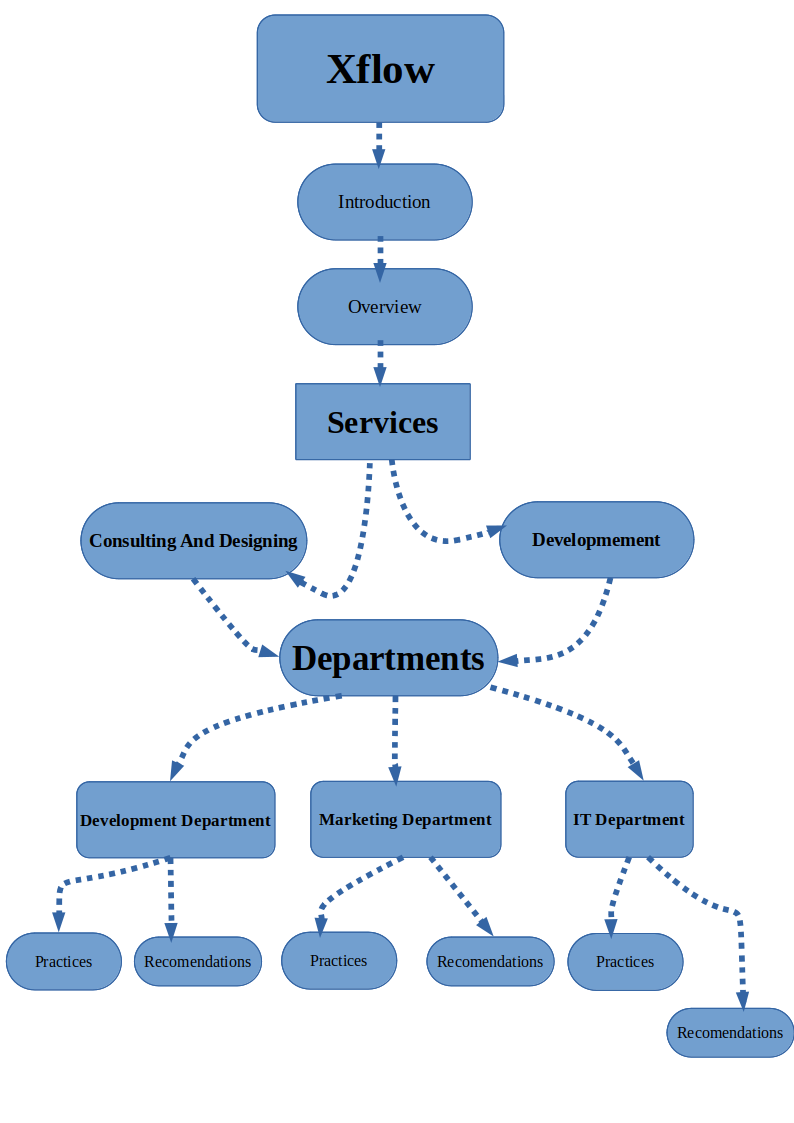
\includegraphics[width=16cm]{draft-2PNG.png}
\end{document}

